%
% main.tex -- Paper zum Thema wwt
%
% (c) 2019 Michael Schmid, Hochschule Rapperswil
%
\chapter{Wetter-Wavelet-Transformation\label{chapter:wwt}}
\lhead{Wetter-Wavelet-Transformation}
\begin{refsection}
\chapterauthor{Michael Schmid}



\definecolor{codegreen}{rgb}{0,0.6,0}
\definecolor{codegray}{rgb}{0.5,0.5,0.5}
\definecolor{codepurple}{rgb}{0.58,0,0.82}
\definecolor{backcolour}{rgb}{0.95,0.95,0.92}

\lstdefinestyle{mystyle}{
	backgroundcolor=\color{backcolour},   
	commentstyle=\color{codegreen},
	keywordstyle=\color{magenta},
	numberstyle=\tiny\color{codegray},
	stringstyle=\color{codepurple},
	basicstyle=\footnotesize,
	breakatwhitespace=false,         
	breaklines=true,                 
	captionpos=b,                    
	keepspaces=true,                 
	numbers=left,                    
	numbersep=2pt,                  
	showspaces=false,                
	showstringspaces=false,
	showtabs=false,                  
	tabsize=2
}
\lstset{style=mystyle}
\lstdefinestyle{mystyle}{
	morekeywords={cwt,contourf,datetick}
}


\section{Einführung}
\rhead{Einführung}


Seit langen konsultiere ich meine aktuellen Wetterdaten von eher unüblichen Internetseite.
Dabei handelt es sich um eine Privat geführte Wetterstation welche die gemessenen Daten, kostenlos und sehr rudimentär im Internet grafisch darstellt.
Weiter werden die Daten auch tabellarisch zur Verfügung gestellt.
Das Feature welches is bis anhin am regelmässigsten nutze, war die grafische Darstellung der aktuellen Wetterdaten über den Zeitraum der letzten 24 Stunden.
Bei speziellen Ereignissen des Wetters, vielen mir besondere und wiederkehrende Charakteristiken auf.
\\
\\
Nach der Einführung in die Theorie der Wavelets kam mir die Idee, solche Wetterphänomene mittels einer geeigneten Wavelet Transformation zu detektieren.
In diesem Paper wird einerseits auf die theoretischen Grundlagen der angewandten Methoden zurückgegriffen sowie die besprochenen meteorologischen Phänomene kurz erläutert. 
Weiterführend wird auf den eigentlichen Prozess des Papers vertieft eingegangen.
Ein besonderes Augenmerk wird auf die allgemeine Vorgehensweise sowie deren Schwierigkeiten gelegt.
\\




\section{Wetterstation Seegräben}
\rhead{Wetterstation Seegräben}

Die  angesprochene Wetterstation ist eine privat geführte Wetterstation in der Gemeinde Seegräben im Kanton Zürich.

Die Wetterstation ist aus einer DAVIS Vantage Pro2 6153 aufgebaut.
Diese besteht aus einem Thermo- und  Hydrosensor, einem Windgeschwindigkeit und Richtungsmesser sowie einem Regenmesser. 
Durch diese Sensoren werden folgende Daten aufgezeichnet:
\\
\\
\\


\begin{itemize}
	\item \textbf{Aussentemperatur} in Grad Celcius
	\item \textbf{Relative Luftfeuchtigkei} in Prozent
	\item \textbf{Luftdruck} in hPa
	\item \textbf{Windgeschwindigkeit} in Km/h, gemittelt über 5 Minuten
	\item \textbf{Windböen} in Km/h
	\item \textbf{Windrichtung} nach Himmelsrichtung
	\item \textbf{Regenmenge} in l/mm²
\end{itemize}	


Der Thermo- / Hydrosensor liegt zusammen mit dem Regenmengenmesser auf 2 Meter über dem Boden.
Mit einem Abstand von rund 10 Meter zum nächsten Gebäude, werden optimale Messbedingungen geschaffen.
Der Windmesser wurde am First des Gebäudes montiert.
Mit einem Masten werden die Daten 1,5 Meter über dem First gemessen.\cite{online:wss}
Die Daten werden anschliessend mit einer Software von PC-Wetterstation.de weiterverarbeitet und auf eine rudiment\"aren Website Dargestellt.
Mehr zur Verwendung der Wetterdaten im n\"achsten Kapitel.

\section{Datenaufarbeitung}
\rhead{Datenaufarbeitung}
\subsection{Wetter-Archiv}
Als n\"achster Schritt der Vorbereitung zur Wavelet Transformation, war die Aufbereitung der zur Verf\"ugung gestellten Daten der Wetterstation Seegr\"aben.
Dazu musste erst analysiert werden wie die Daten auf der Website dargestellt werden.
In der Sektion des Archiv auf der Website kann man die Wetterdaten im gew\"unschten Zeitraum tabellarisch darstellen lassen.
\subsection{Datenerfassung}
Da f\"ur meine Anwendung eine M\"oglichst genaue Aufl\"osung der jeweiligen Daten erforderlich ist, mussten die Daten im Zeitraum von einem Tag dargestellt werden. 
Dies hatte zur Folge, dass man f\"ur jeden Tag ein Tabelle auf dem Archiv der Website \"offnen musste. 
Da mir die Zeit sowie auch die Lust fehlte jeden einzelnen Tag separat zu \"offnen und die Daten mittels "Copy und Paste" Verfahren in eine Excel-Tabelle einzuf\"ugen, war die Motivation gross, ein Programm zu schreiben welches diese Aufgabe automatisieren sollte.
Als Programmiersprache wurde hierf\"ur Python gewählt.
Wie es so üblich ist mit Python, hat man das Wissen zur Vollendung der Aufgabe nicht sogleich auswendig präsent, doch dank kurzen und gezielten Goolge abfragen sowie besuchen des Stackoverflow Forums konnte der ben"otigte Syntax schnell ausfindig gemacht werden.


Mit der Pandas Library und der Funktion "read\_html"\space konnten die Daten direkt mittels Aufruf aus dem Python Programm von der URL-Seite heruntergeladen werden.
Entscheidend für das Gelingen dieser Teilaufgabe war, dass die URL-Links der einzelnen Tage jeweils regelmässig aufgebaut sind.
Da dies der Fall war, konnten die entsprechenden Link mittels einer einfachen While-Schleife zusammengesetzt werden.
\newpage
Folgend der essenzielle Ausschnitt aus dem Python Code:
\begin{figure}[h]
	\centering
	\lstinputlisting[language=Python,firstline=1,lastline=16,numbers=left,style = mystyle]{papers/wwt/code/get_data.py}
	\caption{Python Codeausschnitt}
	\label{fig:python-code}
\end{figure}

Die Daten konnten als nächster Schritt in einer Excel-Tabelle abgespeichert werden.
Dort folgte der letzte feinschliff, dabei wurden alles überflüssigen Kopfzeilen und Statistiken entfernt.

\subsubsection{Unregelmässigkeiten der Wetterstation}
Bei der Datenerfassung durch das eben beschriebene Python Programm wurden einige Unregelmässigkeiten er Wetterstation Seegräben beobachtet.
Das Programm wird jeweils durch einen Fehler abgebrochen, wenn der angegebene Link nicht abrufbar ist. 
So fiel mir auf, dass unregelmässig auf das Jahr verteilt, gewisse Daten von Tagen fehlen, sprich der Link ist nicht abrufbar.
Wenn man manuell auf der Website nach diesem Tag sucht, wird man auch nicht fündig.
Dies trat teilweise sogar in Abschnitten von mehreren Tagen auf.
Wie sich später herausstellte traten die fehlenden Tagen nicht zu den Zeitpunkten auf welche mich interessierten.

\newpage

\subsection{Datendarstellung}
Die Darstellung der gewonnen Daten konnten einfach mittels Matlab gemacht werden.
Anbei die Plot der Rohdaten aus dem Jahre 2018, wobei nur jeder 10 Messpunkt verwendet wurde.
Diese Rohdaten dienten als Grundlage für alle weiteren Berechnungen. 
\begin{figure}[h]
	\centering
	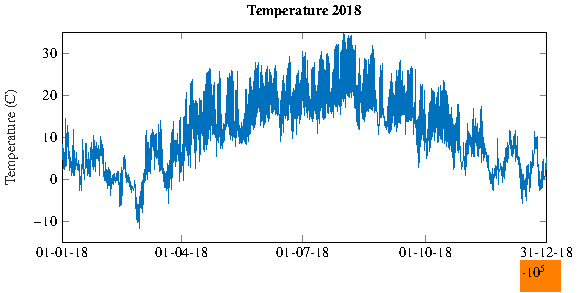
\includegraphics[width=0.9\textwidth]{papers/wwt/images/raw_temp_wwt.pdf}
	\caption{Rohdaten Temperatur 2018}
	\label{fig:rawdata_temp_airp}
	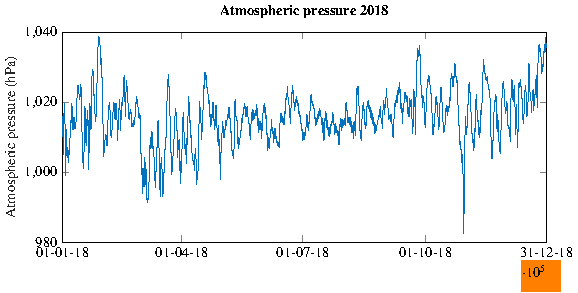
\includegraphics[width=0.9\textwidth]{papers/wwt/images/raw_airp_wwt.pdf}
	\caption{Rohdaten Luftdruck 2018}
	\label{fig:rawdata_temp_airp}
	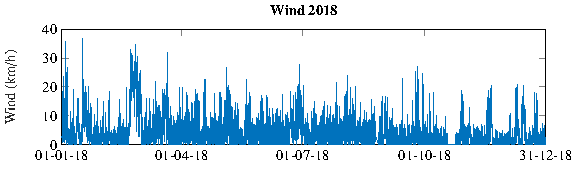
\includegraphics[width=0.9\textwidth]{papers/wwt/images/raw_wind_wwt.pdf}
	\caption{Rohdaten Wind 2018}
	\label{fig:rawdata_temp_airp}
\end{figure}
\begin{figure}[h]
	\centering
	
	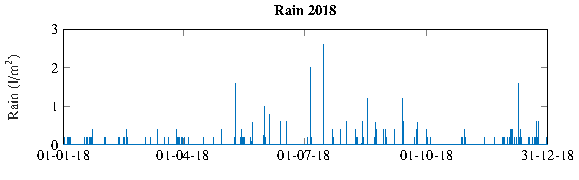
\includegraphics[width=0.9\textwidth]{papers/wwt/images/raw_rain_wwt.pdf}
	\caption{Rohdaten Regen 2018}
	\label{fig:rawdata_wind_rain}
\end{figure}

\newpage
\section{Stetige Wavelet-Transformation}
\rhead{Stetige Wavelet-Transformation}
\subsection{Thoretische Grundlagen}
Die Theoretischen Grundlagen rund um die Stetige Wavelet-Transformation wurde im Kapitel \ref{chapter:cwt} genaustens erläutert. 
In diesem Abschnitt der Seminararbeit wird öfters auf die Theorie des angesprochene Kapitel \ref{chapter:cwt} referenziert ohne diese weiter zu erläutern. 

Für eine m"oglichst genaue Untersuchung der Signalen, in welcher so viele Information gewonnen werden sollten wie m"oglich, eignet sich die Stetige Wavelet-Transformation (folgend noch kurz \textit{cwt} aus dem Englischen "continuous wavelet transform")
ideal. 
Regelmässig auftretende Frequenzen können dank der \textit{cwt} gefunden und zusätzlich auch einem Zeitraum zugeteilt werden.
Darin besteht der allgemeine Vorteil gegenüber der Fourier-Transfomration, denn dort kann man zwar aussagen, dass gewisse Frequenzen auftreten, aber nicht wann diese auftraten.
In 
\begin{equation}
\mathcal{W}f (a,b)
=
\langle f,\psi_{a,b}\rangle
=
\frac{1}{\sqrt{|a|}}\int_{-\infty}^\infty f(t)\,\overline{
	\psi\biggl(\frac{t-b}{a}\biggr)}\,dt
\label{eq:cwt}
\end{equation}

sieht man die Grundlegende Formel der \textit{cwt}.
Wobei das $\psi_{a,b}$ für das Mutter-Wavelet steht, welches mit dem Koeffizienten $a$ skaliert und mit $b$ verschoben wird.

Als Mutter-Wavelet wurde das analytische Gabor-Wavelet verwendet.
\begin{figure}[h]
\centering
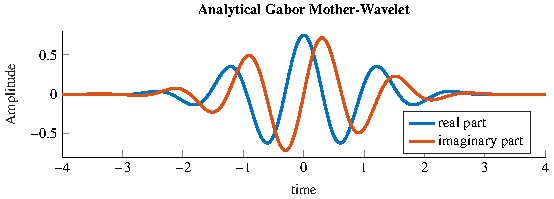
\includegraphics[width=1\textwidth]{papers/wwt/images/gabor.pdf}
\caption{Analytisches Gabor Mutter-Wavelet}
\label{fig:gabor_plot}
\end{figure}

\newpage
\subsection{Berechung mit Matlab}
Die Berechnung der \textit{cwt} wurde mit der numerischen Berechnugs-Software Matlab durchgeführt.
Die essenzielle Funktion dabei war die cwt()-Funktion.
Die Funktion arbeitete bei korrekter Parametrisierung auch wie gewünscht.
Falls man jedoch genauer verstehen möchte wie die Funktion genau rechnet, muss man sich mit einer eher dürftigen Dokumentation herumschlagen.
Glücklicherweise funktionierte die Funktion für meine Anwendung einwandfrei.
Folgende Parameter wurden verwendet
\lstinputlisting[language=Matlab,firstline=1,lastline=1,  numbers=left, style = mystyle]{papers/wwt/code/matlab.m}
\label{fig:matlab_code_cwt}
wobei Matlab das Gabor-Wavelet als 'amor' bezeichnet, mit 'VoicesPerOctave' konnte die Genauigkeit erhöht werden und die Variabel 'fs' beschreibt die Abtastfrequenz der Messsignale.
Bei den Rückgabewerte werden die Wavelet-Werten in 'wt' als komplexe Matrix und die approximierten Frequenzen in 'F' abgespeichert.

Anstatt den Skalierungsfaktor $a$ in \ref{eq:cwt}, wird eine approximierte Frequenz berechnet und zurückgegeben.
Für jeden verwendeten Skalierungsfaktor $a$ wird eine Sinuskurve gesucht, welche am ehesten der Frequenz des entsprechenden Wavelet übereinstimmt.
Siehe in \ref{fig:centerf} ein Beispiel mit einem Daubechies Wavelet der Nummer 7.
\begin{figure}[h]
	\centering
	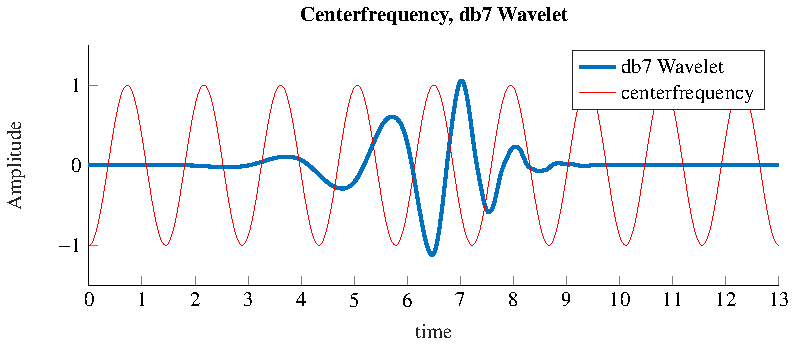
\includegraphics[width=1\textwidth]{papers/wwt/images/centerf.pdf}
	\caption{Approximierte Frequenz eines db7-Wavelet}
	\label{fig:centerf}
\end{figure}


\newpage
\subsection{Verifikation approximierte Frequenz}
Diese approximierte Frequenz konnte man mit den geeigneten Daten aus der aktuellen Anwendung der Wetterdaten sehr gut verifizieren.
Der Temperaturverlauf während einer Hochdruckphase ist sehr regelmässig und man sollte den 24 Stunden Tagesverlauf exakt erkennen.

\begin{figure}[h]
	\centering
	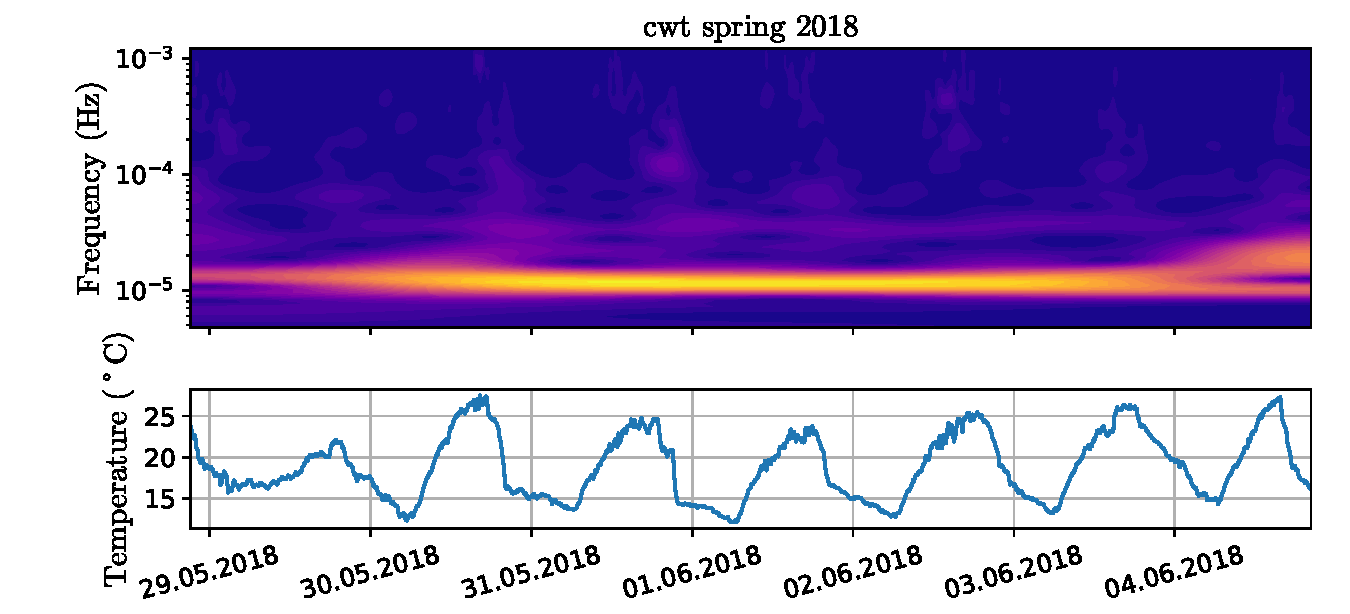
\includegraphics[width=1\textwidth]{papers/wwt/images/data_spring.pdf}
	\caption{Temperaturverlauf und entsp. cwt}
	\label{fig:cwt_zoom}
\end{figure}

Dank der Regelm"assigkeit des Temperaturverlaufs, sieht man im \textit{cwt}-Plot eine signifikante erh"ohung des Wertes bei einer gewissen Frequenz.
Die Ausgelesene Frequenz beträgt $f = 1.16\cdot10^{-5} \,\text{Hz}$, welches umgerechnet einer Periodendauer von $T = 86206.897\,\text{s}\approx 23\,\text{h }56\,\text{min } 47\,\text{s}$ entspricht.
Damit kann die Frequenz im Rückgabewert der Matlab-Funktion als sehr genau betrachtet werden.
Dabei darf nicht vergessen werden, dass nur alle 5 Minuten einen Datenpunkt aufgenommen wurde, und somit die Abweichung zu 24 Stunden kleiner ist als die Auflösung.
Weiter kommt hinzu, dass jeder Tag zu der Jahreszeit im Frühling ca. 2 Minuten kürzer ist als der jeweils Vorgehende.\cite{online:sunset_time}




\section{Analyse von Wettereignissen}
\rhead{Analyse von Wetterereignissen}
Aufgrund der Kenntnissen rund um die \textit{cwt} wurde die Annahme getroffen, dass signifikante Frequenzereignisse gut detektiert werden können.
Bei einer typischen Sturmfront, welche öfters als Wintersturm in den Monaten Dezember und Januar auftreten, zeigten sich bei der Konsultation der Wetterdaten, rapide Temperatur- und Luftdruckwechsel, sowie ein erhöhtes Windaufkommen.
Das Ziel der Analyse war, solche Ereignisse mittels einer geeigneten \textit{cwr} zu detektieren.
\subsection{Sturmsaison 2018}
Bereits bekannt war, dass in der Sturmsaison im Jahre 2018 einige Winterstürme aufgetreten sind.
So wurde bei der Analyse nur auf diese Periode das Augenmerk gelegt.
\\
\\
\\
\\
commit: 26.05.2019



\rhead{Sturmtief}


\section{Schlussfolgerung}
\rhead{Schlussfolgerung}

\printbibliography[heading=subbibliography]
\end{refsection}
